\documentclass{beamer} 

\usepackage[utf8]{inputenc}
\usepackage{graphicx}
\usepackage{multicol}
\usepackage{listings}
\usepackage{pdfpages}


\begin{document}

\title{Using formalism to design secure systems}
\author{Stefan Nožinić (stefan@lugons.org)}

\frame{
\titlepage
}

% https://pdfs.semanticscholar.org/5b26/c71affdd6db82e58344510512d6a2c9f070a.pdf
% https://etd.ohiolink.edu/apexprod/rws_etd/send_file/send?accession=ucin1623169331790079&disposition=inline
% https://www.dsn.kastel.kit.edu/publications/2022-PCN-TLA+.pdf
% https://users.cs.northwestern.edu/~ychen/Papers/Narayana-wimax.pdf
\begin{frame}
    \frametitle{Agenda}
    \begin{itemize}
        \item Motivating example
        \item What are formal specs? 
        \item TLA+ and PlusCal
        \item One real world example
        \item Conclusion
    \end{itemize}

\end{frame}


\begin{frame}
    \frametitle{Process}
    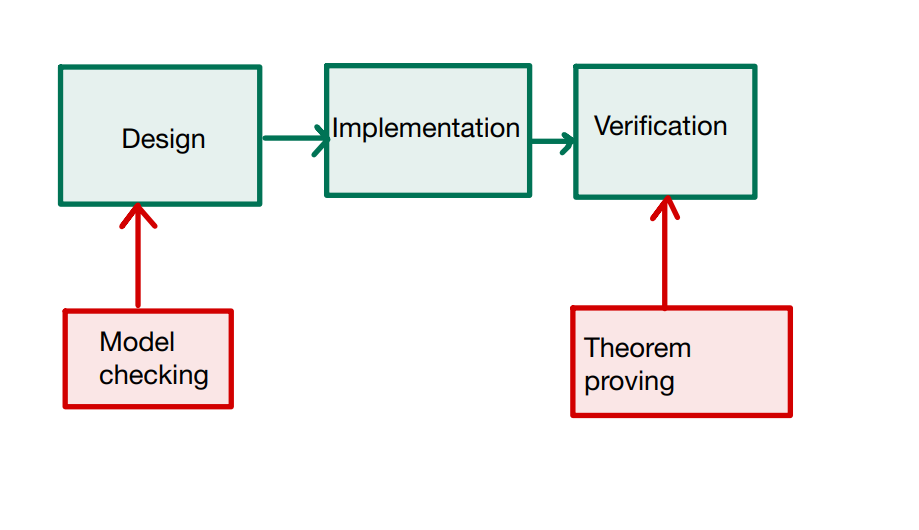
\includegraphics[width=\textwidth]{img/2.png}
\end{frame}

\begin{frame}[fragile]
	\begin{lstlisting}[language=C++]

int main() {
    int i = readInteger();
    i++;
    return 0;
}

	\end{lstlisting}
	
\end{frame}

\begin{frame}
    \begin{center}
        \LARGE{\textbf{How to model this simple program formally as state machine?}}
    \end{center}

\end{frame}

\begin{frame}
    \frametitle{State diagram}
    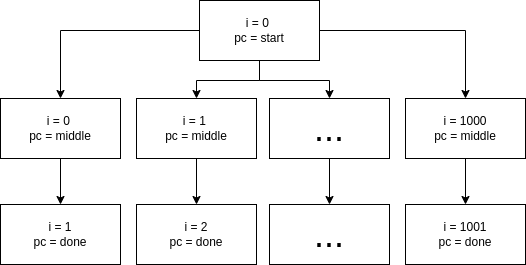
\includegraphics[width=0.9\textwidth, height=0.9\textheight]{img/1.png}
\end{frame}



\begin{frame}[fragile]
    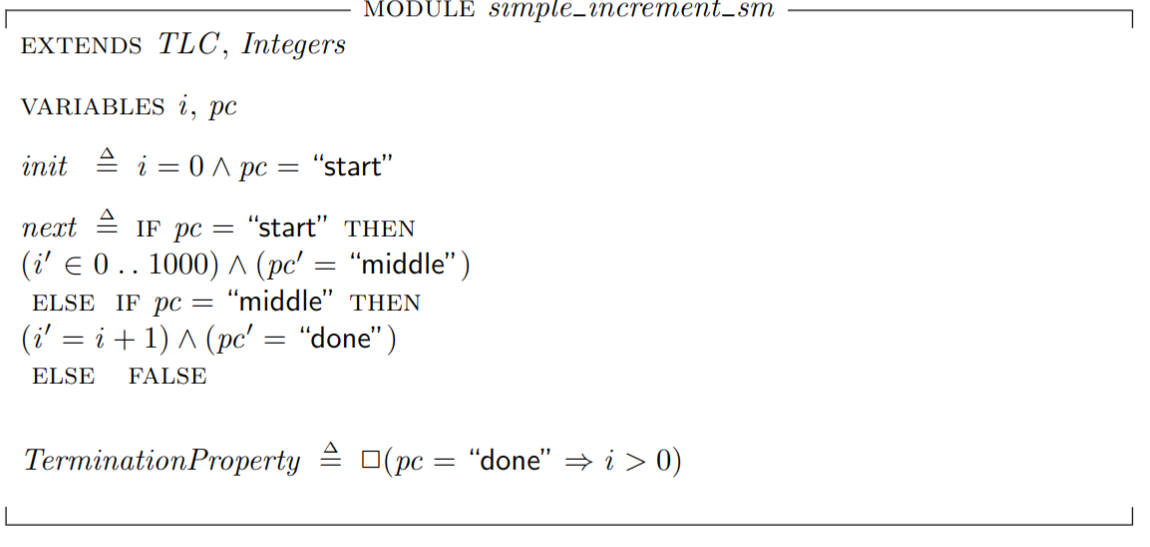
\includegraphics[width=\textwidth]{./sm_increment.png}
\end{frame}

\begin{frame}
    \frametitle{Multiple threads}
\end{frame}

\begin{frame}
    \frametitle{PlusCal}
    \begin{itemize}
        \item A little more progreammer-friendly 
        \item We specify processes and TLC will check all behaviours
    \end{itemize}
\end{frame}


\begin{frame}[fragile]
    \frametitle{Real world example - health monitor}
    \begin{itemize}
        \item We have several nodes (lets say nodes are 1, 2 and 3)
        \item Every node can reboot and recover later on 
        \item Every node has one instance of service called "replicator"
        \item When node is down, its replicator instance gets transferred to another node which is up 
        \item When we detect that replicato instance is stuck, we kill it and restart it 
        \item We state that eventually if replicator is stuck, this will lead to either it being killed or recovered by itself
    \end{itemize}
\end{frame}

\begin{frame}
    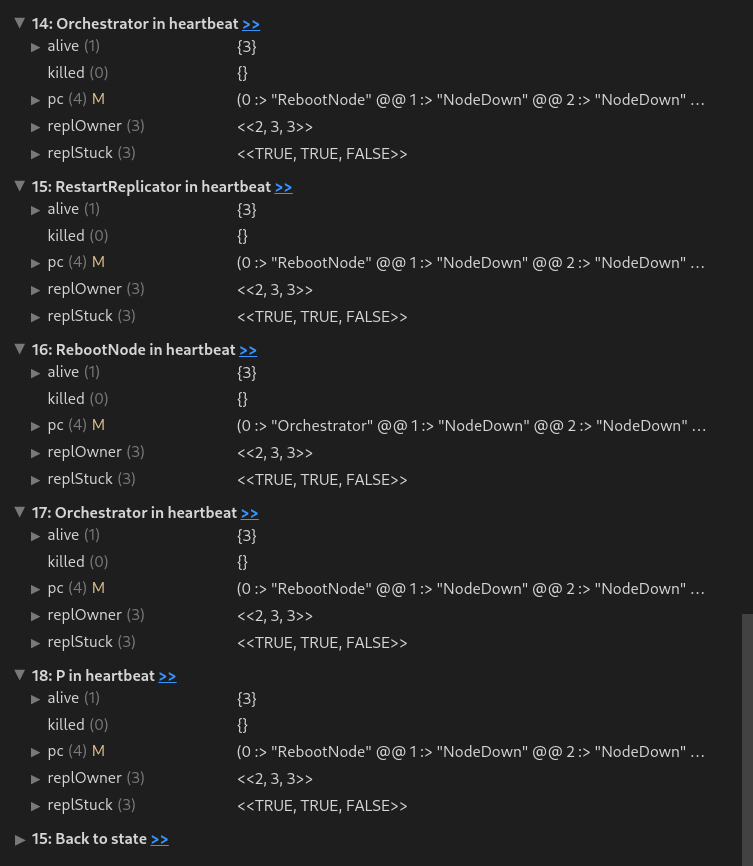
\includegraphics[width=0.9\textwidth, height=0.9\textheight]{examples/img1.png}
\end{frame}


\begin{frame}
    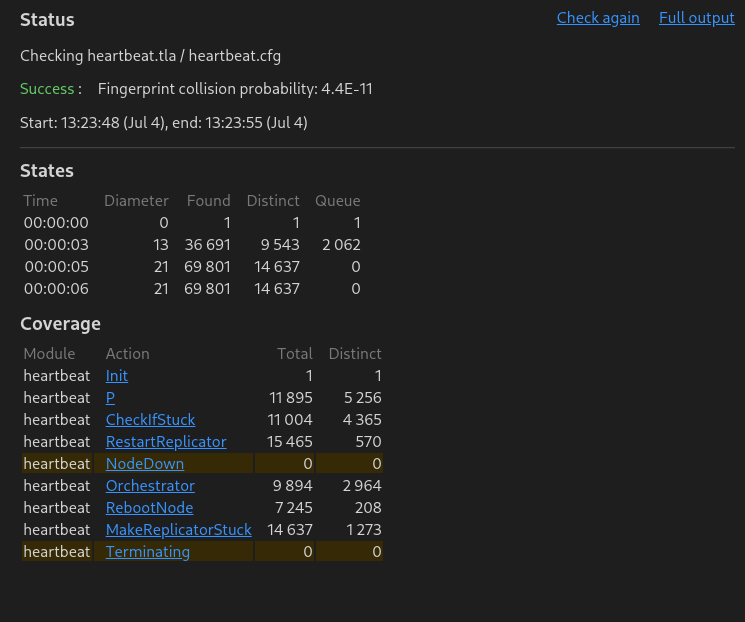
\includegraphics[width=0.9\textwidth, height=0.9\textheight]{examples/img2.png}
\end{frame}


\begin{frame}
    \frametitle{Conclusion}
    \begin{itemize}
        \item Formal specification can help us reason about systems and communicate better in teams
        \item There are tools to help us formally specify systems and to check its validity 
        \item More granular we go, more validation we get
    \end{itemize}
\end{frame}

\begin{frame}
    \begin{center}
        \LARGE{\textbf{Gossip session}}
    \end{center}

\end{frame}

\end{document}
